\documentclass[a4paper]{article}
\usepackage[usenames,dvipsnames]{xcolor}
\usepackage{caption}
\usepackage{subcaption}
\usepackage{listings}
\usepackage{xcolor}
\usepackage{forest}
\usepackage{multicol}
\setlength{\columnsep}{3cm}
\usepackage{parskip}
\usepackage{changepage}
\usepackage[T1]{fontenc}
\usepackage{amsmath}
\usepackage{hyperref}
\usepackage{listings}
\usepackage{amsthm}
\usepackage{amssymb}
\usepackage{float}
\usepackage[utf8]{inputenc}
\usepackage{graphicx}
\usepackage[italian]{babel}
\usepackage{thmtools}
\graphicspath{{figures/}}
\newtheorem*{definition}{Def}
\usepackage{xcolor}
\newcommand{\appunto}[1]{\textcolor{ForestGreen}{#1}}
\newcommand{\R}[0]{\mathbb{R}}
\newcommand{\C}[0]{\mathbb{C}}

\begin{document}

\author{Lorenzo Dentis, lorenzo.dentis@edu.unito.it}
\title{Appunti di Analisi}
\maketitle
\tableofcontents
\newpage
\section{Numeri Complessi}
\subsection{definizione}
\begin{definition}
	Un numero complesso è una coppia ordinata $ (x,y) $ con $ x,y \in \mathbb{R} $.
	Nell' insieme dei numeri complessi $ \mathbb{C} = \{z = x + iy | x,y \in \mathbb{R}\} $ (posti $z_1,z_2 \in \mathbb{C}$) si definiscono le seguenti operazioni.
	\begin{itemize}
		\item[] \textbf{Addizione} $z_1+z_2 = (x_1+x_2, y_1 + y_2)$
		\item[] \textbf{Prodotto} $z_1z_2 = (x_1x_2 - y_1y_2,\; x_1y_2 + x_2y_1) $\\
			\appunto{La "formula" del prodotto si deduce facilmente da $(x_1 + iy_1) (x_2 + iy_2)$}
	\end{itemize}
\end{definition}
Un numero complesso può essere anche scritto in forma algebrica $z= x+iy$.
\begin{definition}
	Dato $z= (x,y)$ definisco "coniugato di $z$": $\overline z = (x,-y)$
\end{definition}
\subsection{proprietà}
Essendo un numero complesso una coppia di numeri reali, si può affermare $\mathbb{C} = \mathbb{R}^2$?\\
Sì,no,sì. 
\begin{itemize}
	\item Insiemisticamente sono uguali \appunto{tanto che spesso si rappresentano i numeri immaginari sul piano di Gauss (piano complesso)} , $z$ è un punto in $\R^2$ di coordinate $(x,y)$
	\item Algebricamente non sono uguali, in quanto il prodotto mostrato in $\mathbb{C}$ non è presente in $\mathbb{R}^2$.
La somma corrisponde alla somma di vettori in $\R^2$ ma il prodotto non ha corrispondenza.
\appunto{il prodotto vettoriale è  completamente diverso in $\mathbb{R}^2$.}
	\item Topologicamente sono uguali, dato un numero complesso $z$, $||z|| = \sqrt{x^2 + y^2}$ chiamata \textit{norma} o \textit{modulo} di $z$. \appunto{cioè la stessa cosa della norma del vettore di coordinate $(x,y) \in \R^2$}.
Da cui deriva che la "distanza" tra due numeri complessi $z,w$ è, \appunto{come in $\R^2$}, $dist(z,w)=||z-w|| = \sqrt{(x_z - x_w)^2 + (y_z - y_w)^2}$

\end{itemize}
Nota: il prodotto fornisce anche una giustificazione alle proprietà dell' \textit{unità immaginaria}
\begin{definition}
	$i=(0,1)$ è detta \textit{unità immaginaria} e verifica formalmente $i^2 =1$
\end{definition}
Infatti $i^2=(0,1)^2 = (0,1)(0,1) = (0*0 -1*1,0*1, 1 *0) = (-1,0) = 1$
\subsection{Altre forme di scrittura}
\begin{align*}
	Z=(x,y) = x+iy = \rho(cos\theta + i sen\theta)=\rho e^{i\theta}\\
	\text{[algebrica]}\quad \text{[alg. in modo trig]}\quad \text{[esponenziale]}
\end{align*}
\subsubsection{Trigonometrica}
Rappresentando sul piano complesso un numero complesso $z$ notiamo che si può esprimere la sua "posizione" anche in coordinate polari.\\
\begin{figure}[H]
	\begin{subfigure}[c]{0.5\textwidth}
	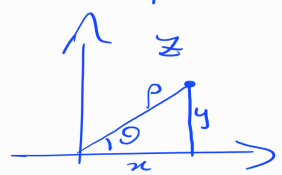
\includegraphics[width=\textwidth]{forma_trig.png}
	\end{subfigure}
	\begin{subfigure}[c]{0.5\textwidth}
		\begin{equation*}
			\begin{cases}
				\rho = \sqrt{x^2 +y^2}\\
				\theta = arctan(\frac{y}{x})
			\end{cases}
		\end{equation*}
		Vivecersa
		\begin{equation*}
			\begin{cases}
				x = \rho cos \theta\\
				y = \rho sin \theta
			\end{cases}
		\end{equation*}
	\end{subfigure}
\end{figure}
$$ z=x + iy = \rho\, cos \theta + i\,\rho \, sin \theta = \rho (cos\theta + i\,sin \theta)$$
Chiamiamo questo modo di esprimere un numero complesso "forma algebrica scritta in modo trigonometrico"

\subsubsection{Esponenzionale}
\begin{definition}[Formula di De Moivre]
	$$e^{i\theta} = cos\theta + i\, sen\theta$$
\end{definition}
Dunque
$$ z = \rho (cos \theta + sen \theta)=  \rho e^{i \theta}$$
\begin{definition}[Esponenziale complesso]\appunto{poco importante}\\
	$$\text{In generale, sia } z = (x,y)$$
	$$e^z = e^xe^{iy}=e^x(cos\,y + i \, sen\,x)$$
\end{definition}
La forma esponenziale permette di svolgere calcoli in maniera più semplice (soprattuto moltiplicazioni e potenze). 
\subsubsection{Note} 
\appunto{poco importanti}\\
Equivalenza tra la scrittura in forme algebrica e la scrittura come coppia di numeri reali.\\
$x = (x,0)\; y=(y,0),\; i=(0,1)$\\ 
$x+iy = (x,0) + (0,1)*(y,0) = (x,0) + (0*y - 1*0, 0*0 + 1*y ) = (x,0) + (0,y) = (x,y)$

Analisi a valori complessi:
Data un funzione $f: \mathbb{I} \rightarrow \C$,  $\forall t\in \mathbb{I},\; f(t)\in \C$
quindi può essere "scomposta": $f(t) = f_1(t) + i\,f_2(t)$.
\appunto{$f_1$ è la parte reale di $f_t$ ed $f_2$ la parte immaginaria}
\begin{definition}[Derivata a valori complessi]
	$$f'(t) = f_1'(t) + i\, f_2'(t)$$
\end{definition}
\begin{definition}[Integrale a valori complessi]
	$$\int_If(t) dt = \int_If_1(t) dt + i\, \int_If_2(t) dt$$
\end{definition}

\section{Segnali e sistemi}
\subsection{Segnali}
\begin{definition}[Segnale]
	Un Segnale è una grandezza fisica variabile nello spazio o nel tempo, rappresentato dalla funzione $f = \R^d \rightarrow \R \; o \; \C$.\\
	Distinguiamo i segnali \textit{analogici} con dominio $\R$ ed i segnali le cui misurazioni sono fatte ad intervalli di tempo (tecnica detta \textit{sampling}) cioè i segnali \textit{analogici} con dominio $\mathbb{Z} \; o \; \mathbb{N}$.
\end{definition}
\begin{figure}[H]
	\begin{subfigure}[c]{0.5\textwidth}
	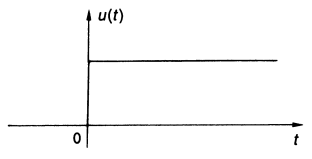
\includegraphics[width=\textwidth]{heavyside_func.png}
\end{subfigure}
	\begin{subfigure}[c]{0.5\textwidth}
		\begin{equation*}
			\mu(t) = 
			\begin{cases}
				0 \qquad se \qquad t<0 \\
				1 \qquad se \qquad t>0 
			\end{cases}
		\end{equation*}
	\end{subfigure}
	\caption{Heavyside function} \label{FIG:heavyside}
\end{figure}
\begin{figure}[H]
	\begin{subfigure}[c]{0.5\textwidth}
	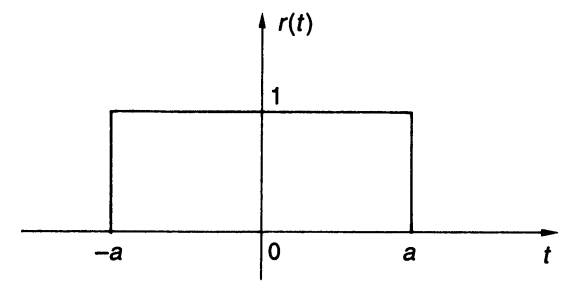
\includegraphics[width=\textwidth]{rectangular_window.png}
	\end{subfigure}
	\begin{subfigure}[c]{0.5\textwidth}
		\begin{equation*}
			r(t) = 
			\begin{cases}
				1 \qquad se \qquad |t|<0 \\
				0 \qquad se \qquad |t|>0 
			\end{cases}
		\end{equation*}
	\end{subfigure}
	\caption{Funzione finestra rettangolare} \label{FIG:rectangular}
\end{figure}
\begin{figure}[H]
	\begin{subfigure}[c]{0.5\textwidth}
	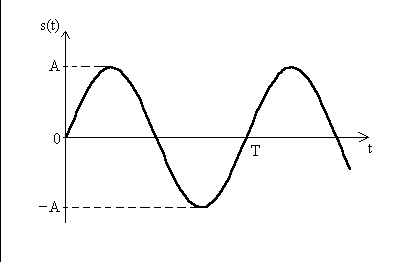
\includegraphics[width=\textwidth]{generic_sin.png}
	\end{subfigure}
	\begin{subfigure}[c]{0.5\textwidth}
		$$x(t) = \alpha cos(2\pi \omega t + \phi)$$
		ove $|\alpha|$ è l'ampiezza, $\omega$ la frequenza (quindi $\frac{1}{\omega}$ il periodo). $\phi$ la fase.
		Identicamente si può esprimere la generica sinusoidie in funzione del seno.
		$$x(t) = \alpha sen(2\pi \omega t + \phi)$$
	\end{subfigure}
	\caption{Sinusoide generica} \label{FIG:generic_sin}
\end{figure}
Le due notazioni possono essere accorpate in un'unica funzione, che, \appunto{grazie alla formula di De Moivre}, può essere riscritta in notazione esponenziale.
$$x(t) = \alpha (cos(\omega t + \phi) + i \; sen ( \omega t + \phi)) = \alpha e^{i(\omega t + \phi)}$$
\appunto{Il $2 \pi$ può tranquillamente essere omesso in quanto costante}

\subsection{Sistemi}
\begin{definition}[Transmission system]
	Un "apparato" che riceve un segnale in input e trasmette un segnali in output.\\ Indicato come $y=A(x)$ o in breve $y=Ax$.
\end{definition}
I sistemi manipolano segnali, quindi prendono in input una funzione e restituiscono in output una differente funzione.
Esempi di semplici sistemi sono: l'amplificatore $y(t) = kx(t)$ con $k$ costante , delayer $y(t) = x(t-a)$ con $a$ costante o il "derivatore" $y(t) = x'(t)$

\subsubsection{Proprietà dei sistemi}
I sistemi possono avere diverse proprietà, quelle che interessano a noi (poichè vanno a definire un \textit{filtro}) sono:
\begin{enumerate}
	\item Linearità: Dato $A: X \rightarrow Y$ $A$ è lineare se:
		$$A(x + y) = A(x) + A(y)$$
		$$A(\lambda x) = \lambda A(x)$$
	\appunto{nota che la seconda condizione deriva in realtà dalla prima}
	\item Causalità: Non può "anticipare i tempi", l'output non può variare prima che vari l'input.
		Formalmente: 
		$$ x_1(t) = x_2(t)\: for \: t<t_0 \Rightarrow Ax_1(t) = Ax_2(t)\: for \: t<t_0 $$
		\appunto{un filtro non deve per forza essere causale, ma per essere realizzabile deve esserlo}
	\item Invarianza alle traslazioni: detta anche "stazionarietà", se traslo temporalmente l'input di $\alpha$ l'output uscirà temporalmente traslato di $\alpha$. 
		Formalmente:
		$$ A(\tau_a x) = \tau_a (Ax)$$
		$\tau$ è un sistema, \textit{delay operator}. Si potrebbe anche scrivere:
		$$ x(t) \rightarrow y(t) \Rightarrow x(t-a) \rightarrow y(t-a)$$
	\item Continuità: Se se segnali di input sono "vicini" allora i due segnali di output sono "vicini" anch'essi. 
		Quando la sequenza di segnali in input $x_n$ tende ad $x$ la sequenza di segnali in output $y_n$ tende a $y$.
		Ma cosa vuol dire che una sequenza di segnali \textit{tende} ad un segnale? 
		Dobbiamo fare riferimento alle norme che approfondiremo nel capitolo dopo \ref{section:norme}, in quanto $x_n \rightarrow x \iff ||x_n - x|| \rightarrow 0$ cioè $x_n$ tende a $x$ se la distanza tra $x_n$ ed $x$ tende a 0. 
		Una definizione formale di Continuità è data al capitolo \ref{sec:continuità}
\end{enumerate}
\begin{definition}
	Un \textbf{filtro} è un sistema che rispetta le proprietà 1,3,4. Un sistema che rispetta anche la proprietà 2 è detto \textbf{Filtro causale}.
\end{definition}
\subsubsection{Norme}
\label{section:norme}
Abbiamo già citato due volte il discorso di norma, ma cosa vuol dire la norma in $\C$ ?
Sia $I in \R $ un intervallo possiamo definire tre norme: 
\begin{enumerate}
	\item \textbf{norma uniforme}: Anche detta norma infinito.
		$$ ||x||_{\infty} = sup|x(t)|$$
		Cioè la norma uniforme di x è il suo estremo superiore.
	\item \textbf{norma 1}: Anche detta norma della media.
		$$ ||x||_1 = \int_I |x(t)| dt$$
		Cioè, ci interessa un valore "normato" del segnale, ottenibile attraverso l'integrale.
		Come in figura \ref{img:norma1_uguale} si può notare che segnali molto differenti possono avere norma 1 uguale.
		\begin{figure}[h]
			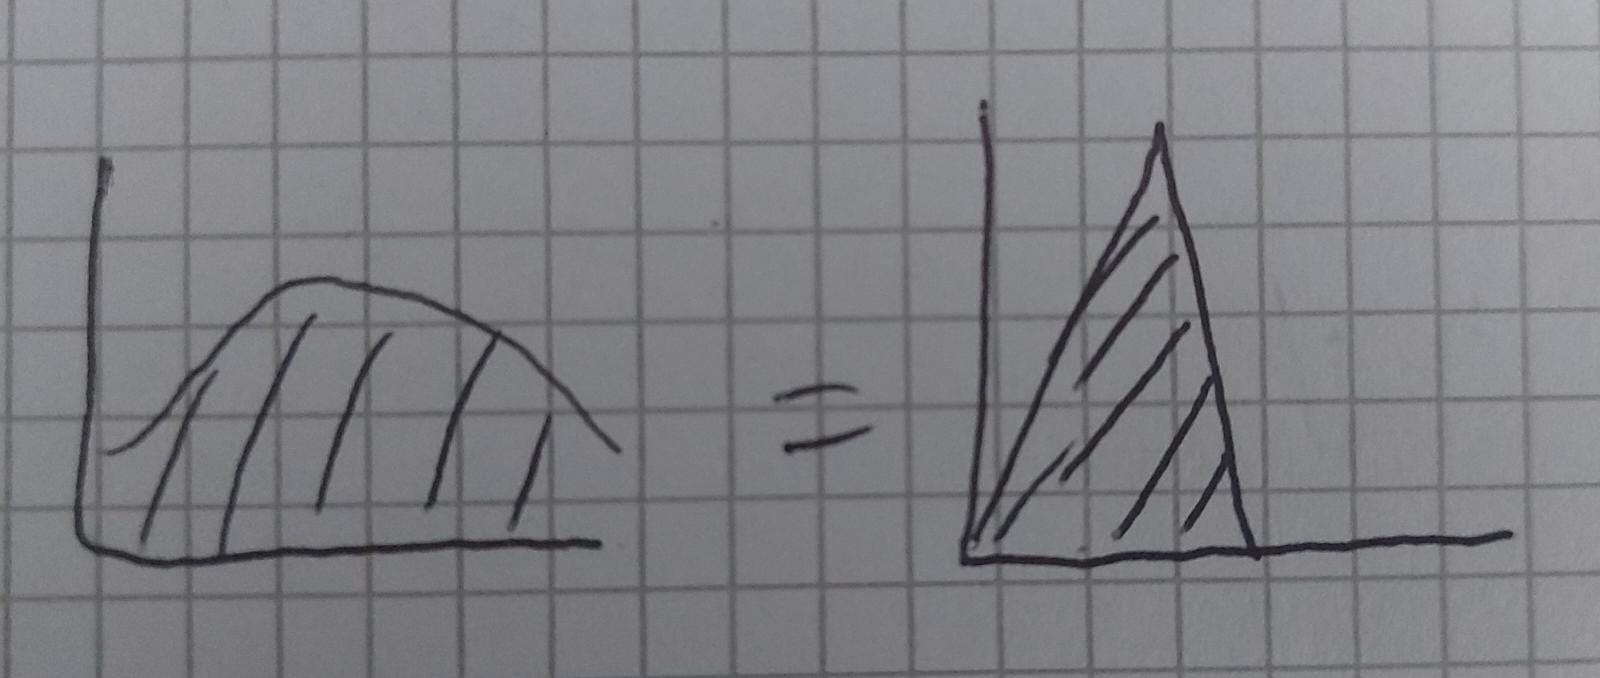
\includegraphics[width=\textwidth]{norma1_uguale.jpeg}
			\caption{due funzioni il cui integrale ha lo stesso valore}
			\label{img:norma1_uguale}
		\end{figure}
	\item \textbf{norma 2}: Norma della media quadratica.
		$$ ||x||_2 = \sqrt{\int_I |x(t)|^2 dt}$$
		Nota: $||x||_2^2$ rappresenta l'energia del segnale.  
		Nota 2: Questa norma in realtà deriva dal prodotto scalare , infatti presi due vettori $u$ e $v$ $u\quad x\quad v = u_1 * v_1+ \quad ... \quad u_n * v_n$ che riscritto nel continuo è
		$$(x,y) = \int_I x(t)\overline{y}(t)dt$$
		E $||x||_2$ non è altro che  $\sqrt{(x,x)}$.
		Posso esprimere la norma 2 come prodotto scalare
\end{enumerate}
Notiamo che nel caso in cui le funzioni da considerare siano discrete possiamo ripetere le dimostrazioni in modo analogo, solo che al posto degli integrali avremo le sommatorie.
\subsubsection{Continuità in norma}
\label{sec:continuità}
Tornando al discorso di \textbf{Continuità}: abbiamo detto \textit{ Quando la sequenza di segnali in input $x_n$ tende ad $x$ la sequenza di segnali in output $y_n$ tende a $y$.}
Adesso che abbiamo la definizione di norma possiamo dire:\\
Il sistema $A : (X, |. . . |_i ) \rightarrow (Y, | . . . |_j )$ \footnote{$X$ indica uno spazio di funzioni, $||...||_i$ indica la norma i-esima che viene usata in $X$ e la coppia $(X,|...|_i)$ è detta \textit{spazio normato}}
è continuo se\\ $\lim_{n\to\infty} ||x_n -x ||_i = 0 \Rightarrow \lim_{n\to\infty} ||y_n - y||_j = 0$ dove $y_n = Ax_n$  e $y = Ax$

\appunto{Nota: un operatore può essere continuo rispetto ad una scelta di norme e non continuo rispetto ad un'altra scelta}
\subsection{Funzione di trasferimeto di un filtro}
Un filtro è un \textit{sitema continuo, lineare ed invariante per traslazioni}.
Data la sua linearità vale che $A(\sum^k_{n=0} a_nx_n)= \sum^k_{n=0} a_nAx_n $.
Ma dato che un filtro è anche continuo possiamo analizzarne il comportamento al limite, quindi:
$$A(\sum^{\infty}_{n=0} a_nx_n)= \sum^{\infty}_{n=0} a_nA(x_n)$$
Inoltre possiamo vedere un segnale come la somma pesate delle frequenze pure che lo compongono, quindi:
$x(t)= \sum^{\infty}_{n=-\infty} c_ne^{2i\pi \lambda nt}$
Dato che $2i\pi$ è una costante e possiamo riscrivere $e^{2i\pi \lambda t}$ come $e_{\lambda}(t)$

Unendo queste due considerazioni possiamo scrivere un filtro come:
$$y=Ax= \sum^{\infty}_{n=-\infty} c_nA(e^n_{\lambda})$$
Cioè descriverlo secondo la sua funzione di trasferimento: una \textbf{funzione delle frequenze} che indica come il filtro attenua o amplifica le varie frequenze.
$f_{\lambda} = Ae_{\lambda} = H(\lambda)e_{\lambda}$
Dato un $e_{\lambda}$ ammissibile come input del filtro A
$$A(e_{\lambda}) = H(\lambda) e_{\lambda}$$

\subsubsection{Filtro passa basso ideale}
Volendo crere un \textit{filtro passa basso}, cioè una funzione che per basse frequenze mantiene un segnale o lo amplifica, mentre impedisce alle alte frequenze il passaggio potremmo definire la seguente funzione $H(\lambda)$:
\begin{equation*}
H(\lambda)=
	\begin{cases}
		3, \text{ se } \lambda < 10.000 \\
		0 \text{  altrimenti}
	\end{cases}
\end{equation*}

\subsubsection{Circuito RC}
\label{sec:circuito_rc}
L'equazione differenziale che regola un circuito è la seguente:
\begin{equation}\label{eq:RC_definition}
RCv'(t) + v(t) = x(t)
\end{equation}
Ponendo $w(t)=v(t)e^{t/RC}$ possiamo riscrivere $v(t)=w(t)e^{-t/RC}$ per poi calcolare $v'(t)$ in modo da ottenere un valore di $w(t)$ dipendente solo da $R,C$ ed $x(s)$

Dopo tanti calcoli che non sto a scrivere (che si possono trovare sugli appunti di Alfano) otteniamo:
\begin{equation} \label{eq:RC}
v(t) = Ax(t)= \frac{1}{RC}\int^t_{-\infty} e ^{-\frac{t-s}{RC}}x(s)ds
\end{equation}
Ove $x$ è il segnale in ingresso ($x(s)$ è la tensione in ingresso al tempo $s$).

Questa espressione definisce un filtro? è lineare ed invariante, è continua?
Ad esempio in norma infinito è continua, per affermare ciò bisogna solo verificare che $||Ax||_{\infty} \leq C||x||_{\infty}$
Con tanti altri calcoli posso dimostrare che 
$\frac{1}{RC}\int^t_{-\infty} e ^{-\frac{t-s}{RC}}x(s)ds \leq ||x||_{\infty}$ e di conseguenza $||Ax||_{\infty} \leq ||x||_{\infty}$ per cui $||Ax||_{\infty} \leq C||x||_{\infty}$

\subsubsection{Convoluzione}
Se definiamo
$$h(t)= \frac{1}{RC}e^{-\frac{t}{RC}}u(t)$$
ove $u(t)$ è la funzione \textit{Heavyside} \ref{FIG:heavyside}
Possiamo riformulare l'equazione \ref{eq:RC}
$$Ax(t) = \int^{\infty}_{-\infty}h(t-s)x(s)dsi=(h*x)(t)$$
L'operazione definita dall'operatore $*$ è detta \textit{convoluzione} tra due segnali, in questo caso $h$ e $x$. \appunto{h contiene al suo interno $R$ e $C$ quindi ci dice come il segnale $x$ viene "trasformato"}

\subsubsection{Funzione di trasferimento filtro RC}
Riprendendo l'eq che definisce il filtro RC \ref{eq:RC_definition} possiamo ottenere la sua funzione di trasferimento.
Quindi il nostro obbiettivo è trovare $h(\lambda)$ che definisce 
$$v(t) = H(\lambda) e_{\lambda}(t)$$
Cioè la funzione che data una frequenza pura del segnale di input descrive come il filtro la modifica.
Sostituendo $v(t)$ nell'eq \ref{eq:RC_definition} otteniamo
$$RC(H(\lambda) e_{\lambda}(t))' +H(\lambda) e_{\lambda}(t) = e_{\lambda}(t)$$
Ricordando che $e_{\lambda} = e^{2i\pi \lambda }$ e derivando la parte dell'equazione che va derivata (\appunto{quella nelle prime parentesi con l'apice}) otteniamo
$$RCH(\lambda) e^{2i\pi \lambda }2i\pi \lambda  + H(\lambda)e^{2i\pi \lambda } = e^{2i\pi \lambda }$$
Raccogliendo $H(\lambda)$ e cancellando un po' di operatori che si elidono otteniamo finalmente
\begin{align*}
	(2i\pi \lambda RC +1) H(\lambda) = 1\\
	H(\lambda) = \frac{1}{2i\pi \lambda RC +1}
\end{align*}
A noi di questa equazione interessa soprattutto il modulo, poichè ci mostra chiaramente che il filtro RC è un filtro passa basso. i segnali con una elevata frequenza (quindi con un $\lambda$ alto) vengono attenuati.
$$|H(\lambda)|^2 = \frac{1}{4i\pi^2 \lambda^2 R^2C^2 +1}\qquad
\footnote{se non tornano i conti è perchè non stai considerando che questo è un numero complesso, quindi il suo modulo è $|a+ib| = \sqrt{a^2 + b^2}$}$$

		\begin{figure}[h]
			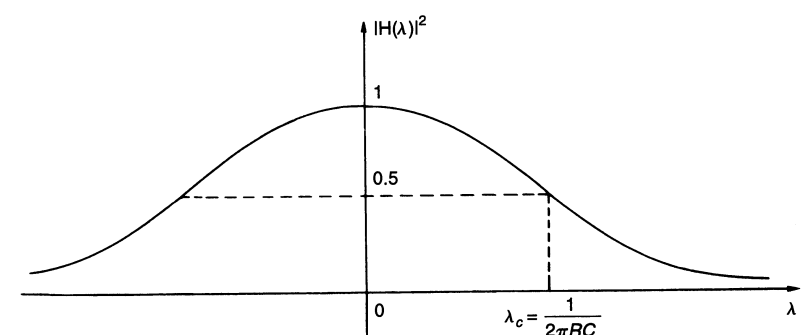
\includegraphics[width=\textwidth]{RC_lowPass.png}
			\caption{Il filtro RC è passa-basso}
		\end{figure}
\end{document}

